\chapter{Python}
\section{Variabel}
\par
Variabel adalah suatu tempat yang berfungsi menampung value dimemori, ibaratkan suatu ruangan atau wadah,  variabel dibagi menjadi dua berdasarkan ruang lingkup yaitu variable lokal dan global, untuk menentukan variabel global atau lokal itu tergantung dari tempat dideklarasikannya variabel pada program yang sedang dibuat. Variabel global yaitu variabel yang dapat diakses di semua lingkup  dalam program yang sedang dibuat, dalam kata lain variabel global ini dapat dikenali oleh semua fungsi dan prosedur, sementara variabel lokal yaitu variabel yang dapat diakses hanya di lingkup khusus, dalam kata lain variabel lokal ini hanya bisa diakses pada fungsi/prosedur dimana variabel itu dideklarasikan.\\ \\
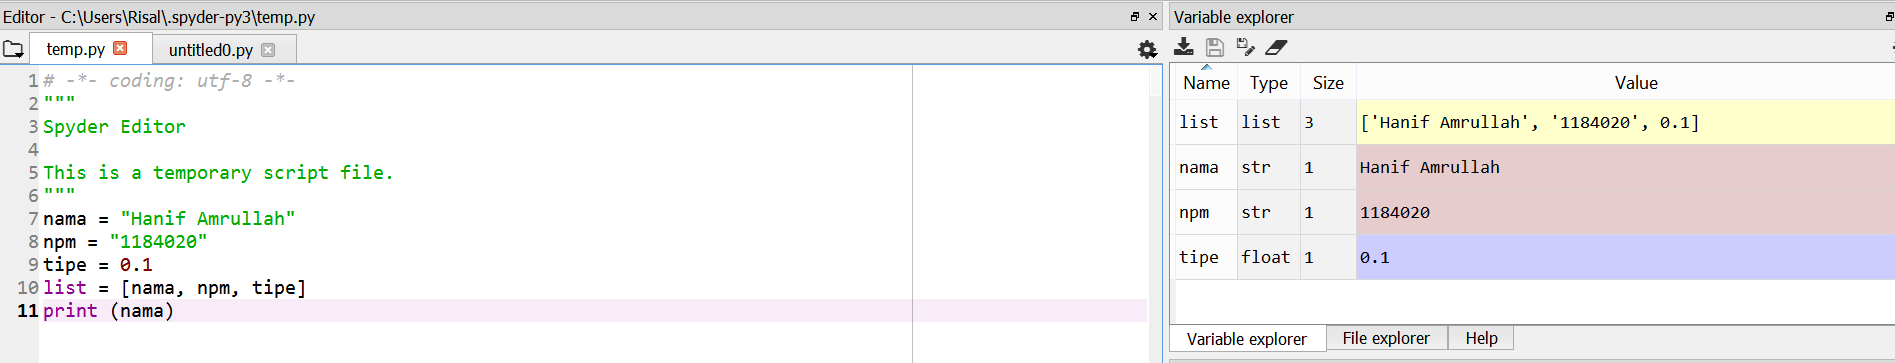
\includegraphics[scale=0.7]{figures/variabel.png} 
        \section{Input dan Output}
        Input dimaksud disini adalah menuliskan kode yang membuat user menginputkan sebuah nilai yang mana nilai tersebut akan memiliki output tersendiri, seperti berikut listing ~\ref{inputoutput}
      
        \lstinputlisting[caption={Input dan Output}, label={inputoutput}, language=Python, firstline=1, lastline=3]{src/InputOutput.py}
        
        \section{Contoh Pemakaian Operator Dasar Aritmatika dan Pengubahan Tipe Data}
        Contoh pemakaian operator dasar aritmatika \ref{aritmatika}
        \lstinputlisting[caption={Operator Aritmatika}, label={aritmatika}, language=Python, firstline=1, lastline=11]{src/Aritmatika.py}
        untuk pengubahan dari tipe data varchar ke integer dapat menggunakan fungsi int() dan harus dipastikan didalam string tersebut harus berisi angka tidak boleh simbol, dan abjad. Seperti di listing \ref{aritmatika},
        
        \section{Perulangan}
        Contoh perintah perulangan pada python ada 3 yaitu \textbf{for, while, dan nested} ketiganya berbeda tetapi fungsinya tetap sama yaitu mengulang suatu perintah yang berada di dalam sintaks looping dengan parameter tertentu untuk membuat looping.

        \subsection{\textit{for}}
        For biasanya digunakan untuk perulangan yang parameter ditentukan langsung. \ref{for}
        \lstinputlisting[caption={For Loop}, label={for}, language=Python, firstline=1, lastline=2]{src/For.py}
        Diatas program akan mengeprint sebuah list \ref{for} yg berupa "Alvian sangat wkwkw" dari 0 sampai dengan 7.

        \subsection{\textit{while}}
        While akan melakukan pengulangan terus menerus jikalau parameter yang dikembalikan bernilai true, contoh pada listing \ref{while}
        \lstinputlisting[caption={While Loop}, label={while}, language=Python, firstline=1, lastline=5]{src/while.py}
        Program diatas akan melakukan pengulangan terus menerus hingga variabel "y" berisi False jika False maka looping dari while ada berhenti.

        \subsection{\textit{nested If}}
        Nested adalah suatu pengulangan yang memungkinkan memasukkan parameter pada sebuah pengulangan, contoh pada listing \ref{nested}
        \lstinputlisting[caption={Nested Loop}, label={nested}, language=Python, firstline=1, lastline=7]{src/nestedif.py}
        Program diatas kita melihat 2 kondisi dan dilakukan perintah dan akan menghasilkan outputan nested if.

        \section{Percabangan}
        Percabangan merupakan algoritma yang menentukan sebuah paramater apakah True apakah False.
        \lstinputlisting[caption={Percabangan If dan If Bersarang}, label={if}, language=Python, firstline=1, lastline=10]{src/if.py}
        
        Program Diatas melakukan kondisi dimana nama \textbf{alvian} merupakan kondisi awal, dan if pertama menyatakan jika ada namanya maka akan \textbf{yap tepat ada nama} kemudian kondisi if ke 2, apabila nama sama dengan \textbf{alvian} maka akan di cetak \textbf{anak kelas D4 TI 2C} apabila salah maka akan dicetak \textbf{bukan Anak kelas D4 TI 2C} apabila kedua kondisi if diatas tidak benar makan akan dicetak \textbf{jadi anda siapa ?}.
        
        \section{Kesalahan yang Sering Terjadi}
        Kesalahan yang sering terjadi dalam melakukan semua perintah diatas yaitu biasanya terjadi yaitu:
        
        \begin{enumerate}
        \item pertama,    if umur < 16:
        NameError: name 'umur' is not defined 
        Pastikan Kondisi nya benar.
        \item TypeError: can only concatenate str (not "int") to str\\
    	penanganan error ini bisa ditangani menggunakan casting operand kedua menjadi string.
    	\end{enumerate}
        \section{Try Except}
        Try except adalah cara untuk menangani suatu eror didalam python. cara menggunakannya ialah:\\
        setiap angka yang dibagi dengan 0 maka akan terjadi eror sudah ketentuannya seperti contoh dibawah ini:\\
x=0\\
try\\
x = 5/0\\

except exception, e:\\
print e\\
\\
\\
print x+1\\
maka akan muncul integer division or modulo by zero 1\\
\\
\\
seharusnya kode diatas tidak dapat dieksekusi tetapi karena menggunakan try except kode diatas dapat dieksekusi walaupun hasilnya akan eror.

        
\chapter{Latihan soal}
\section{Soal}
\subsection{Soal 1}
\lstinputlisting[language=Python]{src/1.soal.py}
\subsection{Soal 2}
\lstinputlisting[language=Python]{src/2.soal.py}
\subsection{Soal 3}
\lstinputlisting[language=Python]{src/3.soal.py}
\subsection{Soal 4}
\lstinputlisting[language=Python]{src/4.soal.py}
\subsection{Soal 5}
\lstinputlisting[language=Python]{src/5.soal.py}
\subsection{Soal 6}
\lstinputlisting[language=Python]{src/6.soal.py}
\subsection{Soal 7}
\lstinputlisting[language=Python]{src/7.soal.py}
\subsection{Soal 8}
\lstinputlisting[language=Python]{src/8.soal.py}
\subsection{Soal 9}
\lstinputlisting[language=Python]{src/9.soal.py}
\subsection{Soal 10}
\lstinputlisting[language=Python]{src/10.soal.py}
\subsection{Soal 11}
\lstinputlisting[language=Python]{src/11.soal.py}
\subsection{Soal 2err}
\lstinputlisting[language=Python]{src/2err.py}

\par LINK YOUTUBE
\par https://www.youtube.com/channel/UCaK61CPlJs5GdyX2KWizf5w/videos?view_as=subscri\pra ber
